
\newcommand{\kms}{\textless k_s(t) \textgreater}
\newcommand{\kmss}{\textless k_s^2(t) \textgreater}
\chapter{Modèle de l'attachement préférentiel en faveur des ``pauvres''}
\begin{minipage}{\textwidth}
	\linespread{1.2}
	\minitoc
\end{minipage}

\section{Introduction}
L'étude de l'évolution des réseaux complexes a connu un intérêt croissant durant les dérnières années, grâce au 
développement de modèles qui reflètent certaines propriétés des réseaux réels, par utilisation des techniques
de la  mécanique statistique, de la théorie des graphes et des simulations numériques 
\cite{BA1999,AB2002,Dorogovtsev-Mendes2002,Newman2003}. L'une des propriétés les plus importantes
étudiée dans ces réseaux est la distribution des degrés, qui est la probabilité $P(k)$ qu'un nœud ait un degré $k$.
On  distingue trois lois principales de la distribution des degrés: loi de Poisson où 
$P(k)=e^{-\langle k\rangle}\frac{\langle k\rangle^k}{k!}$, loi de puissance $P(k)\approx k^{-\gamma}$
où $\gamma$ est l'exposant caractéristique, et la loi exponentielle $P(k)\approx e^{-\frac{k}{c}}$ où
$c$ est une constante.\\
Il semble que, dans la nature, la plupart des réseaux suivent les deux dernières lois de distribution 
mentionnées ci-dessus. Barab\'{a}si-Albert (BA) a réinventé le réseau de distribution des degrés 
sans échelle de Price \cite{Price}. Ce dernier a  remarqué en $1965$ que le nombre de liens vers des articles 
scientifiques, c'est-à-dire le nombre de citations  qu'ils reçoivent, suit une loi de puissance, et donc le 
réseau de citations est sans échelle. Price n'a cependant pas utilisé le terme réseau sans échelle, qui n'a été 
inventé que quelques décennies plus tard par BA.\\
BA a introduit un modèle simplifié basé à la fois sur la croissance et 
l'attachement préférentiel. L'évolution du réseau consiste à commencer avec $m_0$ noeuds connectés, et à
chaque instant un nouveau noeud est introduit dans le réseau et se connecte à $m$ noeuds déjà bien connectés
dans le réseau. Cet attachement préférentiel se réalise avec la probabilité 
$\Pi(k_i)=\frac{k_i}{\sum_j k_j}$, où $i$ est l'un des $m$ noeuds choisis pour se connecter au nouveau noeud 
et $k_i$ est son degré.
Cette probabilité se traduit par le fait que les noeuds les plus connectés auraient
toujours plus de chances de se connecter aux nouveaux noeuds, ou selon le principe de Pareto \cite{Pareto1897}, les riches 
deviennent encore plus riche ``rich get richer''.\\
Comme nous l'avons déjà signalé (voir la section $1.5.2$), les réseaux sans échelle sont largement 
observés dans une variété de systèmes. Cependant, il existe d'autres réseaux réels
qui suivent une loi exponentielle, par exemple, le Réseau mondial de transport maritime 
\cite{ Deng-al2009}, le réseau élctrique des USA \cite{Albert-al2004}, réseaux de neurones
des C.elegans \cite{Achacoso-Yamamoto1992} et le réseau de messagerie à
l'Université de Rovira i Virgili (ENURV ) en Espagne \cite{Albert-al2004}.\\
On croit que la distribution des degrés d'un réseau complexe en croissance, suit 
une loi exponentielle, lorsque les nouveaux nœuds ajoutés au réseau sont liés aléatoirement avec une probabilité uniforme
aux noeuds déjà existants. D'autre part, la loi de puissance se manifeste lorsque les nœuds 
ajoutés au réseau sont liés à des nœuds déjà bien connectés avec la probabilité d'attachement préférentielle.\\
De nombreuses idées sur la formation des réseaux ont été examinées. Par exemple, Barab\'{a}si 
a affirmé que l'attachement préférentiel et la croissance sont tous les deux nécessaires  pour générer un réseau sans échelle \cite{BA-al1999}. Actuellement, on sait que la croissance n'est pas
nécessaire pour un tel objectif, et que un réseau statique avec un nombre de noeuds fixe peut 
avoir une distribution de degré en loi de puissance \cite{Xie-al2008}.
En outre, il est intuitif, que l'attachement préférentiel 
sans l'effet "rich get richer" ne génère pas un réseau sans échelle \cite{Samalam}.
Krapivsky et al \cite{Krapivsky-al2000} ont étudié l'attachement préférentiel non linéaire
avec $\Pi(k_i)\varpropto k^{\gamma}$ et ils ont montré que pour $\gamma<1$, la distribution des degrés suit une loi
exponentielle.\\
Malgré de nombreux efforts, une théorie cohérente et rigoureuse des réseaux en croissance n'est pas encore établie, et 
il n'y a pas encore de principe général pour prédire la topologie finale d'un réseau en évolution. Dans le but de comprendre 
la  formation  et l'évolution des réseaux complexes, plusieurs modèles ont été introduits pour étudier les processus
microscopiques impliqués dans les réseaux en formation. %\cite{Il faut ajouter des références des modèles étudiés dans la litérature}.
\\
Dans ce contexte, on introduit dans ce chapitre un modèle de réseau  complexe qui croît avec un mécanisme 
d'attachement préférentiel favorisant les noeuds les moins connectés.
L'objectif est de vérifier d'une part si la distribution des degrés en loi de puissance persiste en l'absence du 
mécanisme "rich get richer" et d'étudier, d'autre part,  les différences microscopiques entre les 
réseaux sans échelle (hétérogènes) et les réseaux homogènes. \\
Avant d'aborder notre modèle, nous allons traiter en détail le modèle de BA, ce qui permettera d'introduire les différentes
méthodes et techniques essentielles dans nos calculs.   


\section{Les processus dynamiques: théorie et simulation}

\subsection{Introduction}

Cette section est destinée à  donner une brève introduction à la théorie et à la modélisation des processus dynamiques et stationnaires des réseaux, et à définir les approches et techniques de base. En particulier, on va introduire le formalisme de l'équation maîtresse (EM).\\
En général, la solution de EM n'est pas facile même pour des processus dynamiques très simples. Pour cette raison, 
nous présentons des techniques qu'ont va utiliser au long de cette thèse, telles que les approximations déterministes du champ moyen, qui représentent  des approches pour comprendre les caractéristiques qualitatives du processus étudié, et la modélisation avec la méthode de Monte Carlo qui est généralement implémentéé dans des simulations numériques à grande échelle.\\ 
Le but de ces différentes méthodes théoriques est de fournir un cadre général pour démontrer comment les interactions
microscopiques entre les éléments du système conduisent à des phénomènes coopératifs et à l'émergence des propriétés 
des processus dynamiques. Cette stratégie, allant de l'interaction microscopique aux phénomènes collectifs émergents,
a ses racines dans la méthodologie de la physique statistique,  et elle est actuellement
considérée comme un paradigme général pour combler l'écart entre les propriétés locales et les propriétés à grande échelle des systèmes complexes.
\subsection{Équation maîtresse}
Le nom "équation maîtresse" a été inventé à l'origine par Nordsieck, Lamb et Uhlenbeck \cite{Nordsieck-al1940} dans leur étude du modèle Furry des averses de pluie cosmiques \cite{Furry1937}. Peu de temps auparavant, Feller a appliqué une équation de la même structure à la croissance des populations \cite{Feller1939}, et Delbrück à des réactions chimiques auto-catalytiques bien mélangées \cite{Delbruck1940}. Pour plus de détails voir cles références \cite{Kampen2007,Gardiner2009,Weber-Frey2017}.\\
La description dynamique du système est obtenue en introduisant pour chaque constituant $i$ la variable correspondante $\sigma_i$, qui décrit un attribut particulier de i, et caractérise son état dynamique. Nous pouvons énumérer tous les états possibles $\sigma_i=1, 2,. . ., m$ pour chaque constituant, on désigne alors une configuration particulière du système à l'instant $t$ par l'ensemble $\sigma(t)=[\sigma_1(t),\sigma_2(t),\sigma_3(t), ...,\sigma_n(t)]$, où l'indice $i = 1,. . ., n$ parcourt tous les constituants du système de taille $n$.\\
L'évolution dynamique du système est simplement donnée par la dynamique de la configuration $\sigma(t)$ dans l'espace des phases du système, définie par toutes les configurations possibles. Le processus dynamique est décrit par les transitions d'un état $\sigma^a$ vers un autre état $\sigma^b$. En général, il est impossible de suivre la dynamique microscopique des systèmes à grande échelle en raison du grand nombre de variables et de la nature stochastique de la plupart des phénomènes. Pour cette raison, la description dynamique de base du système repose sur l'approche de EM que nous allons brièvement introduire.\\
L'approche EM se concentre sur l'étude de la probabilité $P(\sigma,t)$ de trouver le système à l'instant t dans une configuration donnée $\sigma$. Cette probabilité doit être normalisée, $\sum_{\sigma}P(\sigma,t)=1$, et fournit une description probabiliste du système qui donne les informations les plus pertinentes:
\begin{equation}
\frac{\partial P(\sigma,t)}{\partial t}=\sum_{\sigma'}[P(\sigma',t)W(\sigma'\rightarrow \sigma)-P(\sigma,t)W(\sigma\rightarrow \sigma')],
\end{equation}
où la somme s'exécute sur toutes les configurations possibles $\sigma$ et les termes $W(\sigma'\rightarrow \sigma)$ représentent les taux de transition de la configuration $\sigma'$ vers la configuration $\sigma$ en raison de la dynamique microscopique du système.\\ 
Les EM et les simulations basées sur elles, sont maintenant utilisées dans de nombreux domaines de recherche. Elles sont appliquées dans les contextes de la dynamique de spin \cite{Glauber1963,Kawasaki1966-1,Kawasaki1966-2,Kawasaki1966-3}, des réseaux régulateurs de gènes \cite{Walczak-al2009,Rao-al2002,Tsimring2014}, de la propagation des maladies \cite{Bailey1950,Rock2014}, de l'homéostasie épidermique \cite{Clayton-al2007}, et les processus sociaux et économiques \cite{Weidlich-Braun1992}. Les processus de file d'attente sont souvent modélisés en termes d'EM, mais dans ce contexte, les équations sont généralement appelées équations de Kolmogorov \cite{Gross-al2008}.\\ 
\subsection{Modélisation et simulations numériques}
La simulation numérique a commencé dans les années cinquante lorsque les ordinateurs ont été utilisés pour la première fois à des fins pacifiques, en particulier, l'ordinateur MANIAC a commencé en 1952 à Los Alamos. La simulation fournit une approche complémentaire aux méthodes théoriques. Les domaines de la physique où les approches perturbatives sont efficaces (gaz dilués, vibrations dans les solides quasi-harmoniques) ne nécessitent pas de méthodes de simulation. Inversement, la physique des états liquides, où peu de résultats exacts sont connus et où les développements théoriques ne sont pas toujours sous contrôle, a été développée en grande partie par simulation. La première simulation de liquides par la méthode Monte Carlo a été réalisée par Metropolis et al. en 1953.\\
Dans des modèles plus complexes, même l'approche déterministe pourrait ne pas conduire à des équations résolubles. De plus, ce cadre théorique, intrinsèquement, ne prend pas en compte l'hétérogénéité individuelle ou d'autres fluctuations possibles. L'intégration numérique sur l'ordinateur des équations obtenues ne fournit donc pas une image complète du système. Dans cette situation, des modèles informatiques microscopiques, peuvent être appliqués, dans ces approches, chaque élément individuel est supposé être dans l'un des états possibles. \`{A} chaque pas de temps, la procédure de mise à jour spécifique au modèle qui dépend de la dynamique microscopique est appliquée à chaque élément, ce qui modifie son état en fonction de l'état de ses voisins ou d'autres règles dynamiques. Notamment, la stochasticité du modèle peut être introduite en utilisant des simulations Monte Carlo dans lesquelles les taux et les probabilités sont établis dans l'ordinateur avec l'utilisation de générateurs de nombres aléatoires. La perspective microscopique de cette approche est évidente dans le fait que l'on peut suivre la dynamique de chaque élément individuel. De plus, la dynamique du système se situe au niveau des interactions microscopiques entre les éléments, et les régularités statistiques et les propriétés macroscopiques du système sont étudiées en regardant les quantités globales ou moyennes. L'ordinateur est donc utilisé comme un laboratoire pour étudier des réalités complexes non accessibles mathématiquement ou expérimentalement.
\begin{sloppypar}
	\section{L'évolution dynamique et l'attachement préférentiel dans les réseaux réels}
\end{sloppypar}

\subsection{L'évolution dynamique}
Le modèle de réseau aléatoire ER, suppose qu'on a toujours un nombre fixe de nœuds, $n$. Pourtant, dans les réseaux réels, le nombre de nœuds ne cesse de croître grâce à l'ajout de nouveaux nœuds, par exemple, En $1991$, le WWW avait un seul nœud, la première page Web construite par Tim Berners-Lee, le créateur du Web. Aujourd'hui, le Web a plus d'un trillion ($10^{12}$) de documents, un nombre extraordinaire qui a été atteint grâce à l'ajout continu de nouveaux documents par des millions d'individus et d'institutions (voir Fig.~\ref{hosts}), ainsi que le réseau d'acteurs qui continue à se développer \cite{Barabasi2015}.
\begin{figure}[h]
	\centering
	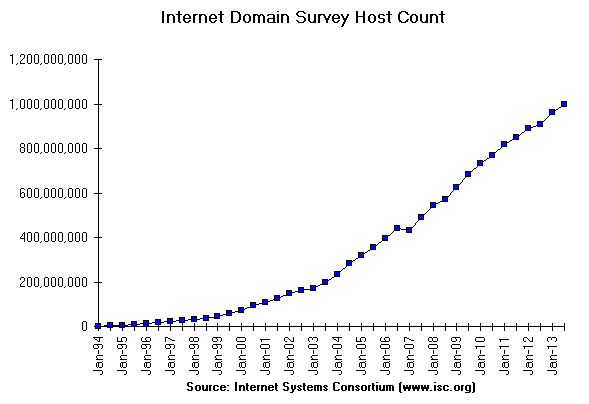
\includegraphics[scale=0.5]{./figures/hosts}
	\caption{L'évolution de nombre d'hôtes sur Interent de $1994$ à $2013$, cette figure  obtenues à partir de site: http://facesncups.com/inforev.html}
	\label{hosts}
\end{figure}
Par conséquent, si nous souhaitons modéliser ces réseaux, nous ne pouvons pas recourir à un modèle statique. Notre approche de modélisation doit plutôt reconnaître que les réseaux sont le produit d'un processus de croissance constant.
\subsection{Le modèle sans échelle BA}

Une caractéristique commune entre le graphe aléatoire ER et les modèles de petit-monde de WS est que la distribution des degrés du réseau est homogène, avec un pic à une valeur moyenne et une décroissance exponentielle, de tels réseaux s'appellent des réseaux exponentiels. Les inconvénients de ces deux modèles précédents est qu'ils ne tiennent pas compte de deux attributs importants de la plupart des réseaux réels.  Premièrement, les réseaux réels sont ouverts et ils sont dynamiquement formés par l'ajout continu de nouveaux nœuds au réseau, par exemple, la WWW génère continuellement de nouvelles pages Web et la littérature de recherche se développe constamment car les nouveaux articles sont en cours de publication. Deuxièmement, le graphe aléatoire ER et le modèle de petit-monde de WS prennent des probabilités uniformes lors de la création de nouvelles arêtes, ce n'est pas réaliste non plus.

Une découverte relativement récente et importante dans le domaine des réseaux complexes est l'observation qu'un certain nombre de réseaux complexes à grande échelle, y compris Internet, WWW, les réseaux métaboliques et plusieurs autres réseaux réels, sont sans échelle et leurs distributions de connectivité ont une forme de puissance (voir Fig.~\ref{scal-free-reels}).\\
Nous nous intéressons à une classe de modèles dont l'objectif principal est de reproduire les processus de croissance qui se déroulent dans des réseaux réels. Nous nous concentrons principalement sur le modèle BA, ce modèle repose sur deux hypothèses simples concernant l'évolution du réseau:
\begin{itemize}
	\item \textbf{Croissance}: De nouveaux nœuds sont ajoutés au réseau, chaque nouveau nœud étant connecté à $m$ des nœuds existants.
	\item \textbf{Attachement préférentiel}: Chaque nouveau nœud est connecté aux nœuds existants avec une probabilité proportionnelle à son degré.
\end{itemize}
De manière plus détaillée, considérons un réseau évoluant dans le temps, $t$, où à chaque fois, un nouveau nœud est ajouté au réseau et connecté à $m$ des nœuds existants, où la probabilité de se connecter à un nœud existant $i$ de degré $k_i$, est donné par:
\begin{equation}
\Pi(i)=\dfrac{k_i}{\sum_jk_j}.
\label{2-2}
\end{equation}
Le nombre de nœuds initial à l'instant $t=0$ est généralement supposé être connecté et doit être supérieur à $m$, mais les détails de sa structure n'ont qu'un faible effet sur le résultat final.\\
Il existe plusieurs méthodes pour analyser les résultats du modèle BA. La méthode la plus simple est une analyse de champ moyen décrite premièrement  dans \cite{BA1999}.
D'autres méthodes plus rigoureuse d'analyse de ce modèle utilisant des outils de la physique statistique comprennent l'approche de l'équation maîtresse \cite{Dorogovtsev-al2000-2} et l'approche de l'équation du taux \cite{Krapivsky-al2000}. La distribution des degrés trouvée est décrite par une loi de puissance avec l'exposant $-3$, c'est-à-dire que la probabilité de trouver un nœud avec le degré $k$ est proportionnelle à $k^{-3}$ (voir Fig.~\ref{BA-distribution}). Afin de trouver l'expression exacte de $P(k)$, nous utilisons l'approche de l'équation maîtresse.\\
Soit $n(k,t)$ le nombre de nœuds de degré $k$ à l'instant $t$. La distribution des degrés $P(k,t)$ se rapporte à cette quantité via la relation $P(k,t)=\frac{n(k,t)}{n(t)}$. Puisque à chaque pas de temps nous ajoutons un nouveau nœud au réseau, nous avons $n=t$. C'est-à-dire qu'à tout moment le nombre total de nœuds est égal au nombre de pas de temps\footnote{En négligeant le nombre des nœuds au temps initial.}.\\
L'attachement préférentiel d'un nouveau nœud avec un ancien nœud dans le réseau de degré $k$ est selon l'Eq.~\eqref{2-2}  comme
\begin{equation}
\Pi(k)=\frac{k}{\sum_{j}k_j}=\frac{k}{2mt},
\end{equation}
où le terme $2m$ représente le fait que dans un réseau, non orienté, chaque lien ajoute deux degrés au réseau. Notre objectif est de calculer les changements dans le nombre de nœuds de degré $k$ après l'ajout d'un nouveau nœud au réseau. Pour cela nous inspectons les deux événements qui modifient $n(k,t)$ et $P(k,t)$ suite à l'arrivée d'un nouveau nœud: le premier est lorsque le nouveau nœud se lie à un nœud  de degré $k$ et il le transforme en un nœud de degré $(k+1)$, ce qui diminue $n(k,t)$, le second lorsque le nouveau nœud se lie à un nœud de degré $(k-1)$ et il le transforme en un nœud de degré $k$, augmentant ainsi $n(k,t)$.\\
Le nombre de liens attendus pour se connecter aux nœuds de degré $k$ après l'arrivée d'un nouveau nœud est $\frac{k}{2mt}\times m\times nP(k,t)=\frac{k}{2}P(k,t)$, autrement dit cette formule représente le nombre des nœuds de degrés $k$ qui acquièrent un nouveau lien et augmente leur degré à $k+1$. De même logique, le nombre des nœuds de degrés $(k-1)$ qui acquièrent un nouveau lien et augmente leur degré à $k$ est $\frac{k-1}{2}P(k-1,t)$.
En combinant ces deux formules présidentes on obtient le nombre attendu de nœuds de degré $k$ après l'ajout d'un nouveau nœud
\begin{equation}
(n+1)P(k,t+1)=nP(k,t)+\frac{k-1}{2}P(k-1,t)-\frac{k}{2}P(k,t).
\label{2-4}
\end{equation}
Cette équation s'applique à tous les nœuds de degré $k>m$. Le fait que nous manquons les nœuds de degré $k<m$ dans le réseau ( car chaque nouveau nœud arrive avec un degré $m$), nous avons alors besoin d'une équation séparée pour le cas de degré $m$. En suivant les mêmes arguments que nous avions suivi pour l'Eq.~\eqref{2-4}, nous obtenons
\begin{equation}
(n+1)P(m,t+1)=nP(m,t)+1-\frac{m}{2}P(m,t).
\label{2-5}
\end{equation}
Notre but est de trouver une distribution stationnaire des degrés. Cela nous pousse à supposer que dans la limite $n=t\longrightarrow \infty$, $P(k,\infty)=P(k)$. En utilisant cela nous pouvons écrire à partir de l'Eq.~\eqref{2-4} et l'Eq.~\eqref{2-5} que
\begin{equation}
P(k)=\frac{k-1}{k+2}P(k-1) \quad \text{si}\quad k>m,
\label{2-6}
\end{equation}
et pour $k=m$ on obtient
\begin{equation}
P(m)=\frac{2}{m+2}.
\end{equation}
Nous utilisons une approche récursive pour obtenir la distribution des degrés. De l'Eq.~\eqref{2-6} on peut écrire
\begin{align}
P(k)&=\frac{k-1}{k+2}P(k-1)\nonumber\\
&=\frac{(k-1)(k-2)}{(k+2)(k+1)}P(k-2)\nonumber\\
&\vdots\nonumber\\
&=\frac{(k-1)(k-2)...(m+1)m}{(k+2)(k+1)...(m+4)(m+3)}P(m)\nonumber\\
&=\frac{(m+2)(m+1)m}{(k+2)(k+1)k}P(m),
\end{align}
de l'équation précédente et sachant que $P(m)=\frac{2}{m+2}$, on obtient l'expression finale de la distribution des degrés dans le modèle BA,
\begin{equation}
P(k)=\dfrac{2m(m+1)}{k(k+1)(k+2)}.
\label{pk-1}
\end{equation}
\begin{figure}[h!]
	\centering
	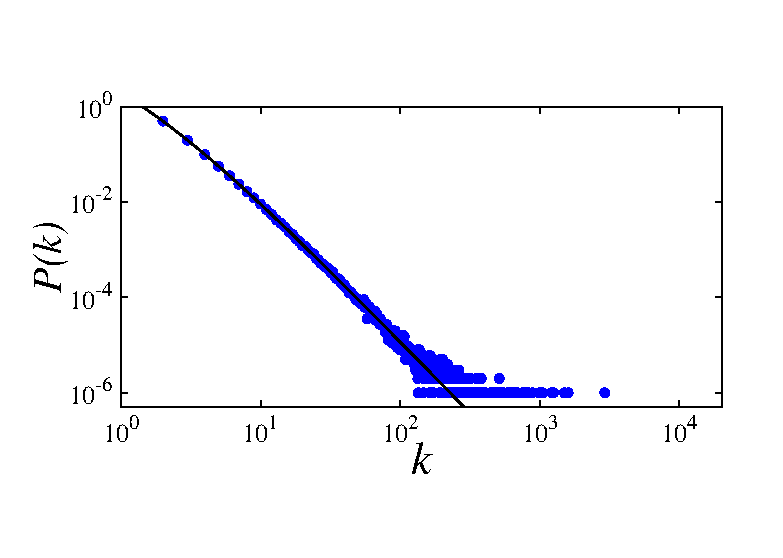
\includegraphics[scale=1]{./figures/fig-barabasi}
	\caption{La distribution des degrés du réseau BA en échelle logarithmique, où les cercles sont les simulations numériques et la ligne continue représente la formule théorique, Eq.~\eqref{pk-1}. La taille du réseau est $\mathrm{n}=10^{6}$ et $\mathrm{m}=2$ .}	
	\label{BA-distribution}
\end{figure}
L'Eq.~\eqref{pk-1} a d'abord été dérivée par Krapivsky et al. \cite{Krapivsky-al2000} et de manière indépendante par Dorogovtsev et al. \cite{Dorogovtsev-al2000-2}. Un traitement plus détaillé a ensuite été donné par Bollobas et al. \cite{Bollobas-Riordan2002}, qui clarifie précisément le domaine de validité de la solution et les écarts éventuels par rapport à la valeur attendue de  $P(k)$.\\ 
La distance moyenne dans le modèle BA est plus petite que dans le graphe aléatoire ER. Les résultats analytiques prédisent une correction de double logarithmique qui diminue la dépendance logarithmique $ L\sim\frac{\log n}{\log\log n }$ \cite{Bollobas-Riordan2002}. Le coefficient de regroupement décroît avec la taille du système comme $C\sim n^{-0,75}$. Il s'agit d'une décroissance plus lente que celle observée pour les graphes aléatoires, $C\sim n^{-1}$, mais le comportement reste différent par rapport aux modèles du petit monde, où $C$ est une constante indépendante de la taille du réseau $n$.
%\begin{sloppypar}
	\subsection{L'attachement préférentielle et le mécanisme "rich get richer"}
%\end{sloppypar}
Le modèle des réseaux aléatoires suppose que nous choisissons au hasard les partenaires d'interaction d'un nœud. 
Pourtant, dans la plupart des réseaux réels les nouveaux nœuds préfèrent se lier aux nœuds les plus connectés, 
ce processus est appelé attachement préférentiel. Par exemple, nous ne connaissons qu'une infime fraction du trillion 
ou plus de documents disponibles sur le WWW. Les nœuds que nous connaissons ne sont pas entièrement aléatoires: nous
avons tous entendu parler de Google et de YouTube, mais nous rencontrons rarement les milliards de nœuds moins
importants qui sont dans le Web. Comme nos connaissances sont biaisées vers les documents Web les plus populaires,
nous sommes plus susceptibles de nous lier à un nœud de haut niveau qu'à un nœud avec seulement quelques liens
\cite{Barabasi2002}.\\
L'ancienneté, cependant, n'est pas suffisante pour expliquer la distribution sans échelle. Les Hubs nécessitent l'aide de 
la deuxième loi, l'attachement préférentiel. Parce que les nouveaux nœuds préfèrent se lier aux nœuds les plus connectés,
les premiers nœuds avec plus de liens seront sélectionnés plus souvent et croîtront plus rapidement que les autres qui 
sont plus jeunes et moins connectés. Comme de plus en plus de nœuds arrivent et continuent de choisir les nœuds les 
plus connectés, les premiers nœuds vont inévitablement se détacher du paquet, acquérant un très grand nombre de liens.
Ils vont se transformer en hubs. Ainsi, l'attachement préférentiel induit un phénomène "rich get richer" qui aide les
nœuds les plus connectés à devenir plus connectés. Alors ce phénomène, "rich get richer", mène naturellement aux distributions sans échelle observées dans les réseaux réels.\\
Dans la section suivante on va introduire un modèle de réseau qui croit avec l'attachement préférentiel, mais en faveur des noeuds les moins connectés, et on va le comparer quantitativement et ``microscopiquement'' avec le modèle de BA.
\begin{sloppypar}
	\section{Attachement préférentiel sans l'effet "rich get richer"}
\end{sloppypar}
%\subsection{Introduction}
\subsection{Le modèle}
Malgré de nombreux efforts, une théorie cohérente et rigoureuse des réseaux en croissance n'est pas encore établie, et 
il n'y a pas encore de principe général pour prédire la topologie finale d'un réseau en évolution. Dans le but de comprendre 
la  formation  et l'évolution des réseaux complexes, plusieurs modèles ont été introduits pour étudier les processus
microscopiques impliqués dans les réseaux en formation %\cite{Il faut ajouter des références des modèles étudiés dans la litérature}.
\\
Dans ce contexte, on introduit un modèle de réseau  complexe qui croît avec un mécanisme 
d'attachement préférentiel favorisant les noeuds les moins connectés.
L'objectif est de vérifier d'une part si la distribution des degrés en loi de puissance persiste en l'absence du 
mécanisme "rich get richer" et d'étudier, d'autre part,  les différences microscopiques entre les 
réseaux sans échelle (hétérogènes) et les réseaux homogènes. 
À l'instar du modèle BA original, notre réseau évolue selon deux mécanismes: la croissance et l'attachement préférentiel. Les nœuds entrants dans le réseau préfèrent s'attacher à des nœuds de faible degré, alors la probabilité $\Pi(k_i)$ que l'un des liens d'un nouveau nœud se connecte au nœud $i$ dépend de son degré $k_i$ tel que $\Pi(k_i)=C(1-\frac{k_i}{\sum_jk_j})$. où $C$ est la constante de normalisation.\\
En ce qui concerne les réseaux sociaux, si nous considérons le degré des nœuds comme décrivant la richesse des gens dans une société capitaliste, nous savons que nous vivons dans un monde où les riches s'enrichissent, mais quelle sorte de société aurons-nous s' il n'y a pas de faveur pour les gens riches, et il y a plutôt une subvention continue pour les pauvres?

Pour mettre en œuvre notre idée, nous commençons par $m_0$ nœuds, chacun avec $m$ liens. À chaque pas de temps, nous ajoutons un nouveau nœud avec $m$ arêtes qui lient le nouveau nœud à $m$ différents nœuds déjà présents dans le réseau. La probabilité que le nouveau nœud soit connecté à un noeud $i$ de degré $k_i$ est $\Pi(k_i)=C(1-\frac{k_i}{\sum_jk_j})$. La constante de normalisation $C$ est déduite de la condition $\sum_{i=1}^{t}\Pi(k_i)=1$, qui donne $C=\frac{1}{t+m_0-1}$. $t$ est l'instant auquel le dernier nœud a été créé et représente également le nombre de nœuds ajoutés au réseau.

\subsection{Distribution des degrés en utilisant l'équation maîtresse}
Notons $n(k,t)$ le nombre de nœuds de degré $k$ à l'instant $t$. La distribution des degrés à un instant donné $t$ sera écrite $P(k,t)=\frac{n(k,t)}{n(t)}$. Puisque à chaque pas de temps nous ajoutons un nouveau nœud au réseau, nous avons $n=t$. C'est, à tout moment, le nombre total de nœuds est égal au nombre de pas de temps.\\
Nous écrivons l'attachement préférentiel dans notre modèle comme
\begin{equation}
\Pi(k)=C\big(1-\frac{k}{\sum_jk_j}\big)=C\big(1-\frac{k}{2mt+mm_0}\big),
\end{equation}
le terme $2m$ capture le fait que chaque lien contribue au degré de deux nœuds, et $mm_0$ capture le fait qu'à l'instant initial nous commençons par $m_0$ nœuds, chacun avec $m$ liens. Notre objectif est de calculer les changements dans le nombre de nœuds de degré $k$ après l'ajout d'un nouveau nœud au réseau. Pour cela, nous respectons les deux événements qui modifient $P(k,t)$ suite à l'arrivée d'un nouveau nœud:
\begin{itemize}
	\item Un nouveau nœud peut être lié à un nœud de degré $k$, le transformant en un nœud de degré $(k+1)$, ce qui diminue $P(k,t)$.
	\item Un nouveau nœud peut être lié à un nœud de degré $(k-1)$, le transformant en un nœud de degré $k$, augmentant ainsi $P(k,t)$.
\end{itemize}
Alors pour ce modèle, l'équation maîtresse peut être écrite comme suit:
\begin{equation}
\begin{aligned}
(t+1)P(k,t+1)= &tP(k,t)+m\Pi(k-1,t)tP(k-1,t)\\
& -m\Pi(k,t)tP(k,t)+\delta_{k,m},
\end{aligned}
\end{equation}
où $\delta$ est le symbole Kronecker.\\
L'équation stationnaire correspondante prend la forme suivante:

\begin{equation}
\begin{aligned}
(t+1)P(k)= &tP(k)+m\big(1-\dfrac{k-1}{2mt+mm_0}\big)\dfrac{tP(k-1)}{t-1}\\
&-m\big(1-\dfrac{k}{2mt+mm_0}\big)\dfrac{tP(k)}{t-1} +\delta_{k,m},
\end{aligned}
\end{equation}
pour des temps très grand on peut écrire que $t+1=t$ et $t-1=t$, d'où
\begin{equation}
P(k)\big(1+m\big(1-\dfrac{k}{2mt+mm_0}\big)\big)=m\big(1-\dfrac{k-1}{2mt+mm_0}\big)P(k-1) +\delta_{k,m},
\end{equation}
après quelque lignes on obtient facilement que:
\begin{align}
P(k)&= 
\begin{cases}
\dfrac{2mt - (k-1)}{2t + 2mt - k}P(k-1), \quad \textrm{for }  k>m,\\
\\
\dfrac{2t}{2t + 2mt - m}, \quad\textrm{for }  k=m.
\end{cases}
\end{align}
La relation de récurrence ci-dessus donne la solution suivante:
\begin{align}
P(k)&= 
\begin{cases}
\dfrac{2t}{2t + 2mt - m}\prod^k_{j=m+1}\left( \dfrac{2mt -j + 1}{2t + 2mt - j}\right), \quad \textrm{for }  k>m,\\
\\
\dfrac{2t}{2t + 2mt - m}, \quad\textrm{for }  k=m.
\end{cases}
\label{eq4-2}
\end{align}
Bien que cette équation ne soit pas fermée, l'estimation numérique de $ P (k) $ est simple comme le montre la Fig.~\ref{fig1-2}. \\
Nous simulons également le réseau avec des tailles allant jusqu'à $n=2\times10^6$, le nombre initial des nœuds est $m_0=3$ et $m=2$. 
Les résultats de la simulation confirment fortement les résultats analytiques (voir Fig.~\ref{fig1-2}). 

\begin{figure}[h]
	\centering
	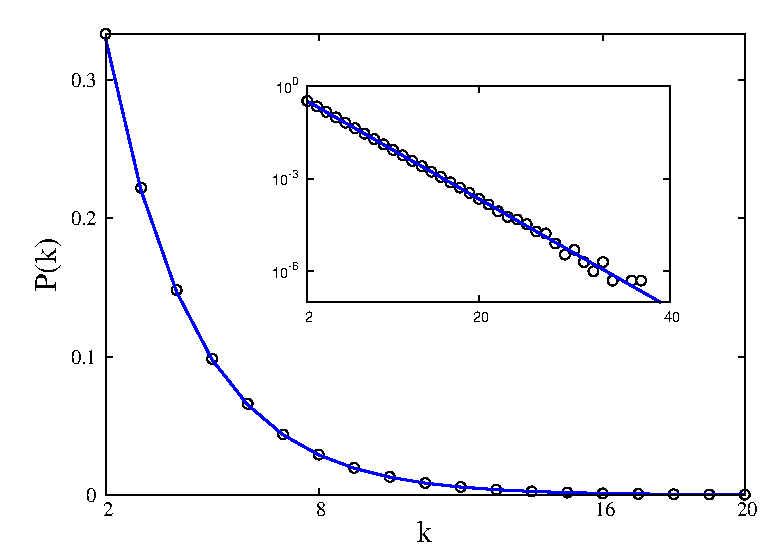
\includegraphics{./figures/fig1}
	\caption{les résultats de la simulation (cercles)  pour $N=2.10^6$, $m=2$, $m_0=3$, et la solution numérique (	ligne continue) pour l'Eq.~\eqref{eq4-2}. Dans l'encart, nous traçons les mêmes données dans l'échelle log-linéaire.}
	\label{fig1-2}
\end{figure} 
Nous avons observé dans les simulations que $k$ reste inférieur à $40$ pour $t=2.10^6$, nous prenons alors $t\gg j $ dans l'Eq.~\eqref{eq4-2} et nous obtenons
\begin{align}
P(k)&\approx 
\begin{cases}
\dfrac{1}{1+m}\Big(\dfrac{m}{1+m}\Big)^{k-m-1}, \quad \textrm{for }  k>m,\\
\\
\dfrac{1}{1+m}, \quad\textrm{for }  k=m.
\end{cases}
\label{eq5-2}
\end{align}
Après la normalisation, nous obtenons la distribution des degrés exponentielle $P(k)=Ae^{-A(k-m)}$, avec $A=\log(\dfrac{m+1}{m})$.
L'encart de la Fig.~\ref{fig1-2} montre la forme exponentielle de $ P(k)$ et l'excellent accord entre les simulations et les résultats théoriques.
Ceci confirme clairement que l'attachement préférentiel seul n'est pas suffisant pour produire des réseaux sans échelle, et il doit y avoir un ``traitement de faveur'' pour les riches pour produire la distribution en loi de puissance. 

\subsection{Comparaison au niveau microscopique avec le modèle de BA}
Nous recherchons les différences entre réseaux hétérogènes et homogènes en comparant notre modèle à celui de BA. La distribution des degrés n'est pas suffisante pour caractériser les réseaux. Le calcul d'autres quantités microscopiques peut aider à mieux comprendre leur évolution et leur formation. Il s'avère que le réseau sans échelle a des nœuds avec un degré important (hubs), tandis que le réseau aléatoire n'a pas de structure apparente. L'évaluation du degré moyen instantané du nœud cible $\kms$ et de ses fluctuations peut fournir des informations quantitatives sur les nœuds du réseau. En fait, $\kms$ est en quelque sorte lié au degré moyen instantané des hubs, car lors du choix aléatoire des nœuds, les hubs ont plus de chance d'être sélectionnés. \\  
Dans un premier temps, nous analysons $\kms$ et $\kmss$ dans le réseau BA
\begin{eqnarray}
\kms=\sum_{t_i=1}^t\Pi(k_i)k_i(t)+m_0\Pi(k_0)k_0(t),
\label{eq6-2}
\end{eqnarray}
où  $\Pi(k_i)=\frac{k_i(t)}{2mt+mm_0}$, $t_i$ est l'instant auquel le nœud $ i $ a été créé, et $ k_0 (t) $ est le degré des nœuds initiaux à l'instant $t$.\\
$k_i (t)$ est facilement calculé à partir de l'équation d'évolution du degré avec le champ moyen:
$\dfrac{\partial k_i(t)}{\partial t}=~ m\Pi(k_i)$, qui donne $k_i(t)=m\Big(\frac{2t+m_0}{2t_i+m_0}\Big)^{\frac{1}{2}}$.\\
En insérant la dernière expression dans l'Eq.~\eqref{eq6-2}, on obtient
\begin{eqnarray}
\kms&=&m\Big(\sum_{t_i=1}^{t}\dfrac{1}{2t_i+m_0}+1\Big) \\
&=&m \Big(\ln (2t+m_0)+\gamma-a+\frac{1}{2(2t+m_0)}+O(\frac{1}{t^2})\Big),
\label{eq7-2}
\end{eqnarray}
où $\gamma$ est la constante d'Euler, et $a=\frac{1}{2}+\frac{1}{3}+\ldots+\frac{1}{1+m_0}$.\\
Un bon accord est obtenu, comme le montre la Fig.~\ref{fig2a-2}, entre l'Eq.~\eqref{eq7-2} et les résultats de la simulation même pour les premiers instants de l'évolution. $\kms$ croît indéfiniment avec le temps et diverge pour un réseau infini ($t\to\infty$) du fait que, dans les réseaux hétérogènes, les hubs sont plus susceptibles d'être sélectionnés et liés aux nouveaux nœuds. \\
De l'autre côté, le degré moyen du réseau reste fini \cite{Barrat-a2008l,Cohen-Havlinl2010} puisque la majorité des nœuds ont un faible degré et le poids des hubs est faible.\\
\begin{figure}[h]
	\centering
	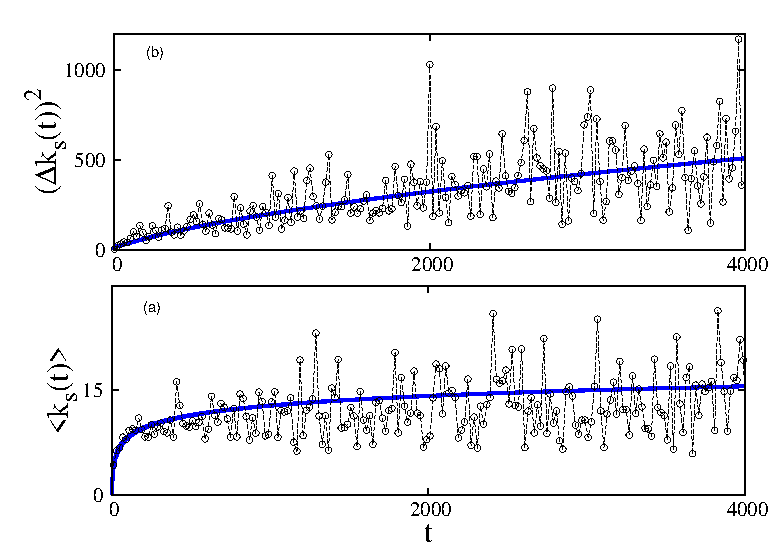
\includegraphics[scale=1]{./figures/nfig2}
	\caption{(a) Évolution de $\kms$ dans le modèle BA, la ligne continue représente l'Eq.~\eqref{eq7-2}.
		(b) Évolution des fluctuations de $\kms$, la ligne continue représente l'Eq.~\eqref{eq10-2}. Les cercles joints par des lignes pointillées dans les deux cas sont des données de simulation moyennées sur 20 réalisations pour $m =2$, $m_0=3$.}
	\label{fig2a-2}
\end{figure}
Le moment d'ordre 2 $\kmss$ s'écrit
\begin{align}
\kmss&=\sum_{t_i=1}^t\Pi(k_i)k^2_i(t)+m_0\Pi(k_0)k_0^2(t)\label{eq8-2} \\
&\approx m^2(2t+m_0)^{\frac{1}{2}} \Big(\sum_{t_i=1}^t \frac{1}{(2t_i+m_0)^{\frac{3}{2}}}+m_0^{-\frac{1}{2}}\Big).
\end{align}
Pour des grands temps, $\sum_{t_i=1}^t\Big(\frac{1}{t_i}\Big)^{\frac{3}{2}}=\zeta(\frac{3}{2}) \approx 2.612$, on obtient 
\begin{eqnarray}
\begin{split}
\kmss&\approx m^2\sqrt{2t}(m_0^{-\frac{1}{2}}+2.612-b),
\label{eq9-2}
\end{split}
\end{eqnarray}
où $b=1+\frac{1}{2^\frac{3}{2}}+\frac{1}{3^\frac{3}{2}}+\ldots+\frac{1}{(1+m_0)^\frac{3}{2}}$.\\
Les fluctuations de $\kms$ sont données par
\begin{align}
(\Delta k_s(t))^2 \equiv \kmss-\kms^2\approx m^2 \Big[(m_0^{-\frac{1}{2}}+2.612-b)\sqrt{2t}-(\ln(2t))^2\Big],
\label{eq10-2}
\end{align}
qui deviennent arbitrairement large lorsque le temps augmente suffisamment. \\
Les données de simulation selon l'Eq.~\eqref{eq10-2} ( voir Fig.~\ref{fig2a-2}(b)) montrent la tendance croissante des fluctuations de $\kms$.
Cela peut s'expliquer par le fait que le degré maximum dans le réseau $k_{max}\sim \sqrt{t}$ \cite{Cohen-Havlinl2010} augmente plus vite que $\kms\sim \ln(t)$ (Eq.~\eqref{eq7-2}) et la différence entre les deux quantités devient plus grande avec le temps. \\
Nous passons maintenant à la même analyse dans notre modèle,  L'équation d'évolution du champ moyen pour $k_i(t)$ est donnée par
\begin{eqnarray}
\dfrac{\partial k_i(t)}{\partial t}=m\Big(1-\dfrac{k_i(t)}{2mt+mm_0}\Big)\dfrac{1}{t+m_0-1}.
\end{eqnarray}
La solution a la forme
\begin{eqnarray}
k_i(t)=m \Big(\frac{t+m_0-1}{2t+m_0}\Big)^{\frac{1}{m_0-2}}\Bigg[\Big(\frac{t_i+m_0-1}{2t_i+m_0}\Big)^{-\frac{1}{m_0-2}}-A(t_i)
+A(t)\Bigg],
\label{kit}
\end{eqnarray}
où $A(t)=\displaystyle \int_1^{t}\dfrac{\Big(\frac{t'+m_0-1}{2t'+m_0}\Big)^{-\frac{1}{m_0-2}}}{t'+m_0-1}dt'$.\\
Or la valeur moyenne du nœud sélectionné $\kms$ est: 
\begin{eqnarray}
\kms=\sum_{t_i=1}^t\Pi(k_i)k_i(t)+m_0\Pi(k_0)k_0(t),
\label{kms-2}
\end{eqnarray}
en remplaçant l'Eq.~\eqref{kit} dans cette dernière équation, on obtient immédiatement pour tout temps $t$ l'expression de $\kms$, L'équation résultante est résolue numériquement comme le montre la Fig.~\ref{fig2b-2}. \\
Pour les temps grands et en prenant $t \gg m_0$, nous trouvons 
$A(t)\approx 2^{\frac{1}{m_0-2}} \ln(t)$, $k_i(t)\approx m\Big(1+\ln \dfrac{t}{t_i}\Big)$, d'où
\begin{align}
\label{kom}
\kms&\approx\dfrac{m}{t}\Big(\sum_{t_i=1}^{t} \ln(t)-\ln(t_i)+1\Big)\\
&\approx\dfrac{m}{t}\Big(t \Big(\ln(t)+1\Big)-\Big(\sum_{t_i=1}^{t} \ln(t_i)\Big)\Big) \nonumber \\
&\approx\dfrac{m}{t}\Big(t\ \Big(\ln(t)+1\Big)-\ln(t_i!)\Big) \nonumber \\
&\approx2m. \nonumber
\end{align}
Le second moment est obtenu en substituant les expressions correspondantes de $\Pi(k_i)$ et $k_i(t)$ dans l'Eq.~\eqref {eq8-2}, nous obtenons pour les temps grands
\begin{eqnarray}
\begin{split}
\kmss\approx \frac{m^2}{t}\Big(\sum_{t_i=1}^t (\ln(\frac{t}{t_i})+1)^2\Big).
\label{k2om}
\end{split}
\end{eqnarray}
En utilisant les approximations  $\sum_{t_i=1}^t \ln(t_i)\approx t\ln(t)-t$, et
$\sum_{t_i=1}^t \ln(t_i)^2\approx t\ln(t)^2-2t\ln(t)+2t-2$, on obtient $\kmss\approx 5m^2.$ L'expression finale des fluctuations est alors 
\begin{eqnarray}
(\Delta k_s(t))^2 \equiv {\kmss-\kms^2}\approx m^2.
\end{eqnarray}
Ce résultat, additionné avec $\kms\approx 2m $, montrent que presque tous les nœuds ont le même degré comme le montre la Fig.~\ref{fig2b-2}. L'homogénéité du réseau peut s'expliquer par le fait que l'attachement préférentiel utilisé ici ne permet pas la formation des hubs, puisqu'il ne permet pas aux riches de s'enrichir encore plus ni aux pauvres de devenir riches. 
\begin{figure}[h]
	\centering
	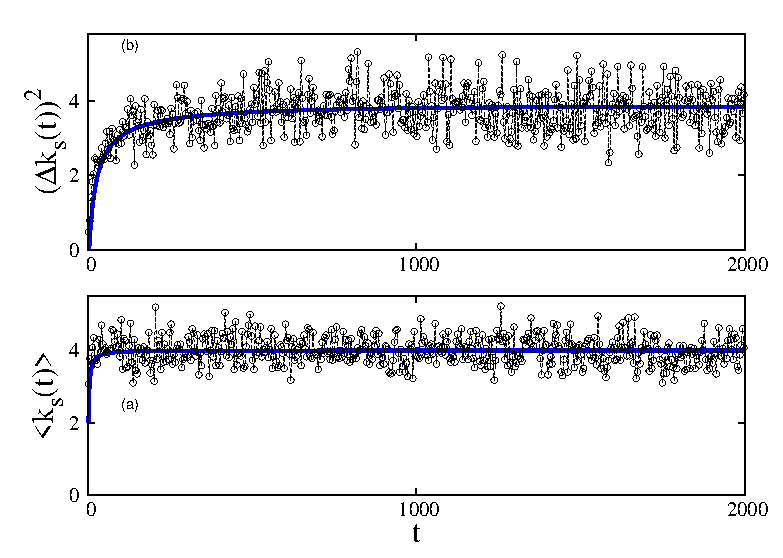
\includegraphics[scale=1]{./figures/nfig3}
	\caption{(a) Évolution de $\kms$ dans notre modèle, la ligne continue représente l'Eq.~\eqref{kms-2}.
		(b) Évolution des fluctuations de $\kms$. La ligne continue représente la solution numérique de l'Eq.~\eqref{kms-2} et de l'Eq.~\eqref{k2om}. Les cercles joints par des lignes pointillées dans les deux cas sont des données de simulation moyennées sur $20$ réalisations pour $m=2$, $m_0=3$.}
	\label{fig2b-2}
\end{figure}
\vspace{4cm}
\section{conclusion}

Dans ce chapitre, nous avons commencé par donner quelques idées sur les processus dynamiques, l'attachement préférentiel et le mécanisme "rich get richer" dans les réseaux réels~, puis nous avons introduit un simple modèle de réseau complexe avec le critère d'attachement préférentiel et sans l'effet "rich get richer". Le réseau obtenu est homogène, ce qui démontre le rôle crucial de l'effet "rich get richer" dans la topologie du réseau. En outre, nous avons conclu que le fait de donner un traitement préférentiel aux nœuds les moins connectés équivaut à utiliser une probabilité d'attachement aléatoire. Le calcul du degré moyen instantané d'un nœud sélectionné et ses fluctuations fournissent plus d'informations que le degré moyen habituel du réseau, en particulier nous avons montré comment le degré moyen des hubs et ses fluctuations divergent avec le temps dans le modèle BA, et restent finis dans notre modèle.
%En termes de répartition de la richesse sociale, le principe de Pareto \cite{Pareto1897} ne s'applique pas et nous avons plutôt une distribution exponentielle du revenu.
\let\cleardoublepage\clearpage
